\documentclass{article}

\usepackage[utf8]{inputenc} 
\usepackage[T1]{fontenc}
\usepackage[french]{babel}
\usepackage[margin=2.5cm]{geometry}
\usepackage{hyperref}
\usepackage{graphicx}
\usepackage[ruled,linesnumbered]{algorithm2e}
\usepackage{xcolor}

\newcommand{\pluseq}{\mathrel{+}=}
\newcommand\comm[1]{\footnotesize\ttfamily\textcolor{gray}{// #1}}

\title{Projet C++ : problème du sac à dos à choix multiple et politique d'incitations}
\author{\textsc{Javaudin} Lucas, \textsc{Le Rest} François}

\begin{document}

\maketitle

\tableofcontents

\newpage

\section{Introduction}

En recherche opérationnelle, le problème du sac à dos\footnote{Voir \url{en.wikipedia.org/wiki/Knapsack_problem}} est un problème d'optimisation dont l'objectif est de maximiser la valeur des objets que l'on insère dans un sac qui ne peut pas supporter plus d'un certain poids.

Nous étudions ici une variante du problème du sac à dos : le problème du sac à dos à choix multiple ou \textit{multiple choice knapsack problem} (MCKP).
Dans le MCKP, les objets sont regroupés en plusieurs classes et le sac à dos doit être rempli avec un et un seul objet de chaque classe.

Le MCKP est un problème NP-complet.
Nous proposons plusieurs algorithmes qui donnent une approximation de la solution optimale.
Plus précisément, les solutions proposées par ces algorithmes sont réalisables et leur distance par rapport à la solution optimale est bornée.

Enfin, nous montrons que le problème du sac à dos à choix multiple est équivalent au problème consistant à trouver la politique d'incitations maximisant l'utilité sociale, lorsque les individus font face à un choix discret et lorsque le budget de la politique est contraint.

\section{Algorithmes}
% On peut mettre ici un pseudo-code des algorithmes que l'on a codé.

\subsection{Recherche exhaustive}

L'algorithme de recherche exhaustive parcourt toutes les allocations possibles et renvoie l'allocation optimale, c'est-à-dire l'allocation qui a la plus grande valeur parmi toutes les allocations dont le poids ne dépasse pas la capacité du sac à dos.

Cet algorithme est NP-hard.
En effet, si l'on note $J$ le nombre de classes et $n$ le nombre d'objets dans chaque classe, alors le nombre d'allocation possible est $n^J$.\footnote{Nos algorithmes autorisent un nombre d'objets différent dans chaque classe. Dans ce cas, le nombre d'allocation possible est $n_1 \cdot \dots \cdot n_J$ où $n_i$ est le nombre d'objets dans la classe $i$.}

Pour parcourir toutes les allocations, on ordonne les objets dans chaque classe et on commence par l'allocation qui prend le premier objet de chaque classe.
Pour obtenir l'allocation suivante, on prend l'objet suivant de la première classe.
Si l'on atteint le dernier objet de la première classe, alors on prend l'objet suivant de la deuxième classe (si ce n'est pas le dernier de la classe), et ainsi de suite.
La table \ref{tab:recherche-exhaustive} montre comment l'algorithme parcourt toutes les allocations lorsque qu'il y a trois classes avec trois objets dans chaque classe (les objets sont indicés 0, 1 et 2).

\begin{table}[!ht]
	\centering
	\caption{Fonctionnement de la recherche d'allocation pour $J=3$ et $n=3$}
	\label{tab:recherche-exhaustive}
	~\\
	\begin{tabular}{c|ccc}
		& Classe 1 & Classe 2 & Classe 3\\
		\hline
		Allocation 1 & 0 & 0 & 0\\
		Allocation 2 & 1 & 0 & 0\\
		Allocation 3 & 2 & 0 & 0\\
		Allocation 4 & 0 & 1 & 0\\
		Allocation 5 & 1 & 1 & 0\\
		Allocation 6 & 2 & 1 & 0\\
		Allocation 7 & 0 & 2 & 0\\
		Allocation 8 & 1 & 2 & 0\\
		Allocation 9 & 2 & 2 & 0\\
		Allocation 10 & 0 & 0 & 1\\
		$\vdots$ & $\vdots$ & $\vdots$ & $\vdots$\\
	\end{tabular}
\end{table}

\begin{algorithm}[!ht]
\caption{Algorithme de recherche exhaustive pour le MCKP.}
\label{alg:recherche-exhaustive}
\small
\SetKwInOut{Input}{Input}\SetKwInOut{Output}{Output}
\Input{$J$ classes avec $n_j$ objets dans chaque classe, capacité $c$}
On note $\mathbf{x} = (x_1, \dots, x_J)$ l'allocation actuelle.\\
Dans chaque classe, on choisit l'objet d'indice 0 : $x_j = 0$, $\forall j$.\\
$\tilde{j}=0$ \comm{Classe modifiée lors de la recherche d'une nouvelle allocation.}\\
$\mathbf{x}^{*} = $ null \comm{Allocation optimale.}\\
$v^{*} = 0$ \comm{Valeur totale de l'allocation optimale.}\\
\While{$\tilde{j} < J$}
{
	\comm{On cherche l'allocation suivante.}\\
	$\tilde{j} = 0$\\
	\While{true}
	{
		\eIf{$x_{\tilde{j}} < n_{\tilde{j}}$}
		{
			On choisit l'objet suivant dans la classe $\tilde{j}$ : $x_{\tilde{j}} \pluseq 1$.\\
			\textbf{break}
		}
		{
			On reprend l'objet d'indice 0 dans la classe $\tilde{j}$ : $x_{\tilde{j}} = 0$.\\
			On s'intéresse à la classe suivante : $\tilde{j} \pluseq 1$.
		}
	}
	\comm{On regarde si la nouvelle allocation est l'allocation optimale.}\\
	$w =$ poids total de l'allocation $\mathbf{x}$\\
	\uIf{$w < c$}
	{
		$v =$ valeur totale de l'allocation $\mathbf{x}$\\
		\uIf{$v > v^{*}$}
		{
			$v^{*} = v$\\
			$\mathbf{x}^{*} = \mathbf{x}$\\
		}
	}
}
\Output{Allocation $\mathbf{x}^{*}$}
\end{algorithm}

\subsection{Algorithme Greedy simple}

\subsection{Algorithme Greedy avec enveloppe convexe}

\subsection{Algorithme Dyer-Zemel}

\section{Structure du code}
% On peut mettre ici un diagramme de classe UML et une présentation des fichiers avec leur contenu.

\begin{figure}[!ht]
	\centering
	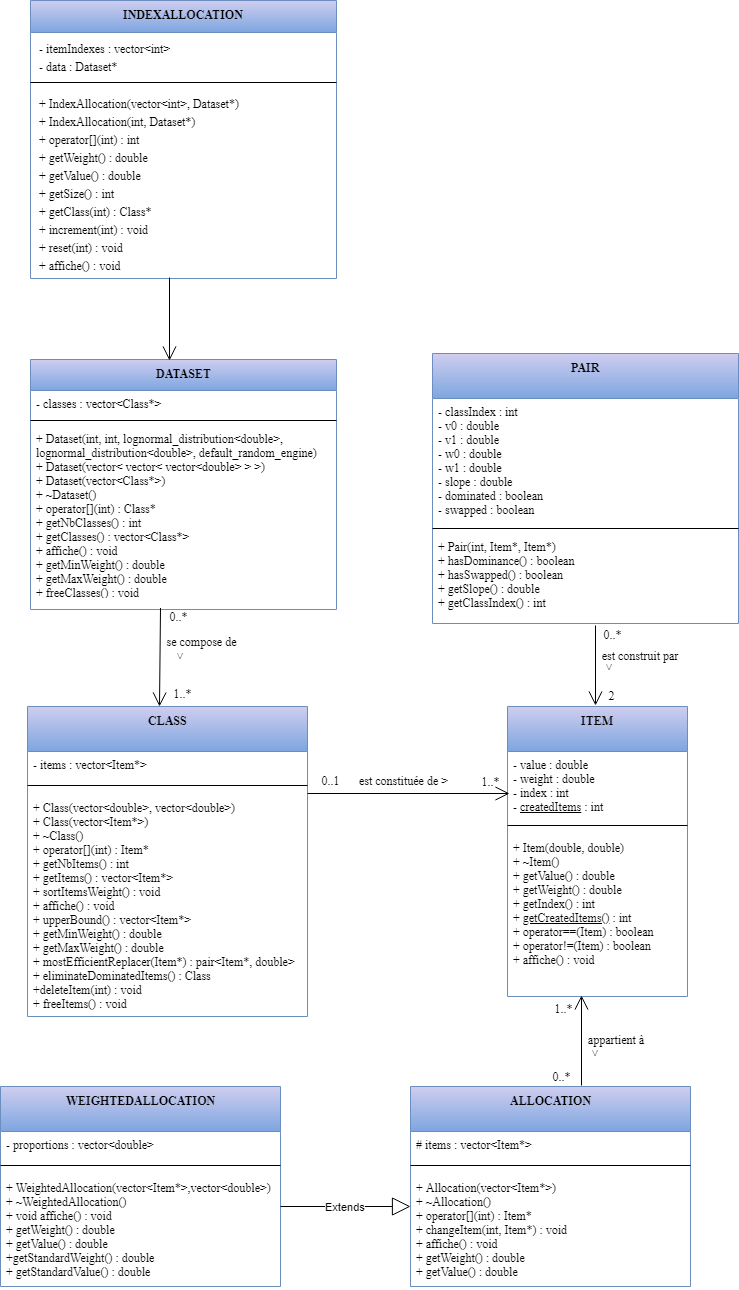
\includegraphics[width=14cm]{KnapsackClasses.png}
	\caption{Diagramme de classes}
	\label{fig:diagramme}
\end{figure}

\section{Application économique}
% Je vais ici parler de l'application du MCKP à une politique d'incitation.

\section{Références}

\begin{thebibliography}{9}
\bibitem{Knapsack2004}
  Hans Kellerer, Ulrich Pferschy and David Pisinger,
  \textit{Knapsack problems},
  Springer,
  2004.
\end{thebibliography}

\end{document}
